% !TeX spellcheck = fa
\documentclass[a4paper,12pt]{report}

\usepackage{color}
\usepackage{xcolor}
\usepackage{fourier}
\usepackage{amsmath}
\usepackage{dirtree}
\usepackage{caption}
\usepackage{verbatim}
\usepackage{fancyhdr}
\usepackage{graphicx}
\usepackage{outlines}
\usepackage{enumitem}
\usepackage{fancyvrb}
\usepackage{subcaption}
\usepackage[Bjornstrup]{fncychap}%Options: Sonny, Lenny, Glenn, Conny, Rejne, Bjarne, Bjornstrup
\usepackage{indentfirst}
\usepackage{listings}
\usepackage{lstautogobble}
\usepackage[colorlinks,linkcolor=blue,citecolor=red,urlcolor=blue]{hyperref}
\usepackage[logo=on,fontsize={12,18}]{xepersian}

%\settextfont{Microsoft Sans Serif}
\settextfont{XB Yas}
\setlatintextfont{Arial}

\definecolor{ao}{rgb}{0.0, 0.5, 0.0}
\definecolor{codeGreen}{rgb}{0, 0.5, 0.5}
\definecolor{lavendergray}{rgb}{0.87, 0.86, 0.92}
\definecolor{mint}{rgb}{0.24, 0.71, 0.54}
\definecolor{aliceblue}{rgb}{0.94, 0.97, 1.0}
\definecolor{customCommentGreen}{rgb}{0.13, 0.65, 0.47}
\definecolor{steelBlue}{rgb}{0.00, 0.00, 0.50}
\definecolor{stringGreen}{rgb}{0, 0.5, 0}

\pagestyle{fancy}

\cfoot{\thepage}
%\rhead{\thepage }

\renewcommand{\headrulewidth}{0.4pt}

\newcommand{\lrInlineMono}[1]{{\color{steelBlue}\lr{\texttt{#1}}}}

\begin{document}
	\lstset{
		frame=tb,
		basicstyle=\color{steelBlue}\linespread{0.8}\ttfamily,
		columns=fullflexible,
		keepspaces=false,
		tabsize=3,
		autogobble,
		breaklines=true,
		breakatwhitespace=true,
		stringstyle=\color{stringGreen},
		commentstyle=\color{gray},
		keywordstyle=\color{purple},
		language=java,
		aboveskip=3mm,
		belowskip=3mm,
		showstringspaces=false,
		columns=flexible,
		captionpos=b,
		numbers=left,
		numbersep=5pt,
		numberstyle=\color{gray}\linespread{0.8}\ttfamily,
		postbreak=\mbox{\textcolor{blue}{$\hookrightarrow$}\space}
	}
	
	\renewcommand{\bibname}{مراجع}
	
	\title{
		\setlatintextfont{XB Titre}
		\lr{Portability and Safety: Java}
	}
	\author{
		سیّد مُرتِضیٰ رَضوی
	}
	\date{
		پنج‌شنبه، ۱۴ فروردین ۱۳۹۹
	}
	
	\maketitle
	\setcounter{page}{384}
	
	\setcounter{chapter}{12}
	\chapter{امنیت و قابلیت‌حمل: جاوا}\label{chap13}
	زبان برنامه‌نویسی جاوا
	\LTRfootnote{\lr{Java.}}
	 توسط آقای جیمز گاسلینگ 
	\footnote{\lr{James Gosling}
		همچنین به عنوان
	\lr{Dr.java}
		شناخته می‌شوند.}
	و چند تن دیگر در شرکت 
	\lr{Sun Microsystems}
	\footnote{شرکت سان میکرو سیستم سازنده رایانه و نرم‌افزار است.}
	طراحی شد.
	این زبان از یک پروژه در سال ۱۹۹۰ بوجود آمد که 
	Oak \footnote{\lr{/əʊk/}
	به معنی بلوط.}
	 نام داشت و بر روی دستگاه‌هایی مورد استفاده قرار گرفت که به عنوان 
	\lr{set-top box}
	 نیز شناخته می‌شدند.
	 
	\lr{set-top box}
	 دستگاه کوچک محاسباتی که به یک شبکه متوسط متصل شده و در بالای یک تلویزیون قرار می‌گیرد. این دستگاه ويژگی‌های زیادی فراهم می‌کند. شما می‌توانید تصور کنید با این فرض که یک مرورگر وب بر روی تلویزیون شما به نمایش درآمده و به جای استفاده از صفحه کلید،شما ‌با استفاده از یک کنترل بر روی آیکون‌های آن کلیک می‌کنید. 
	 ممکن است  شما بخواهید یک برنامه یا فیلم را انتخاب کنید و یا اینکه یک برنامه شبیه ساز کامپیوتر را که توانایی اجرا بر روی یک دستگاه محاسباتی را داشته باشد دانلود و اجرا کنید و آن را به نمایش درآورید. 
	 یا حتی یک تبلیغات تلویزیونی در مورد ماشین می‌تواند با ایجاد یک شبیه سازی منحصر   به فرد رانندگی آن ماشین در جاده در قالب یک تور برای هر بیننده ایجاد کند.
	 هرچند که این سناریو می‌تواند برای شما جذاب باشد، محیط گرافیکی می‌تواند شامل گرافیک، اجرای برنامه‌های ساده و ایجاد ارتباط بین یک سایت و یک برنامه که به صورت داخلی اجرا می‌شود، باشد.
	 
	 در نقطه از توسعه 
	 \lr{Oak}
	  ،مهندسین و مدیران در شرکت سان میکرو سیستم متوجه یک نیاز فوری برای ایجاد یک زبان برنامه نویسی تحت مرورگر  شدند، 
	 یک زبان که می‌توانست برای نوشتن برنامه‌های کوچکی که تحت شبکه متنقل می‌شدند و بر روی هر مرورگر استاندارد در یک پلتفرم استاندارد اجرا می‌شدند استفاده شود.
	و از طرفی نیاز برای استاندارد به دلیل خواسته ذاتی اشخاص و کمپانی‌ها برای داشتن بیشترین مخاطب ممکن بود. علاوه بر قابل حمل بودن، همچنین نیاز به امنیت هم وجود داشت بنابراین کسی که برنامه‌ی کوچکی را دانلود می‌کرد، قادر به اجرای آن بدون ترس از ویروس کامپیوتری یا خطرات دیگر بود.
	
	زبان برنامه نویسی
	\lr{Oak}
  با هدف پیاده سازی دوباره زبان برنامه‌نویسی 
	\lr{C++}
  شروع شد. درحالی که، این طراحی زبان هدف انتهایی پروژه نبود، بلکه تبدیل به تمرکز گروه بر روی آن شد.
  برخی دلایل طراحی یک زبان جدید در این کتاب بیش از حد نمایشی هستند، اما هنوز برخی نقل قول‌های آموزنده از "
	\lr{The Java Saga}"
  توسط دیوید بلانک در 
	\lr{Hot Wierd}\footnote{
  سایت
	\lr{http://www.hotwired.com/}}
	(در دسامبر ۱۹۹۵) موجود است:
	
	\begin{center}
		\fcolorbox{ao}{aliceblue}{%
		\begin{minipage}{.9\linewidth}
			
			%Figure james gsaling
			
			\noindent\textbf{
			جیمز گاسلینگ }
			\\[5mm]		
		جیمز گاسلینگ مهندس ارشد و طراحی کلیدی زبان برنامه نویسی و پلتفرم جاوا بود. او هم‌اکنون در مرکز 
		تحقیقات شرکت سان بر روی ابزار‌های توسعه نرم افزار فعالیت می‌کند. اولین پروژه وی در شرکت سان،  سیستم
		پنجره 
	\lr{NeWS}\footnote{مخفف \lr{Network extensible Window System}.}
		بود که برای 
		\lr{Sun workstation}\footnote{\lr{/sʌn ˈwɝːkˌsteɪʃən/}
		به معنی ایستگاه کاری سان.} در سال ۱۹۸۰ توزیع شده بود.
		قبل از پیوستن وی به شرکت سان، گاسلینگ، یک نسخه چند پردازنده از یونیکس 
		\LTRfootnote{\lr{UNIX /ˈjuːnɪks/.}}
		 ساخت، همچنین سیستم پنجره اندرو
		\LTRfootnote{\lr{Andrew.}}
		به همراه ابزار آن 	 و خیلی از کامپایلر‌ها و سیستم‌های 
		\lr{mail}.
		همچنین او در نظر افراد زیادی سازنده ویرایشگر
		 \lr{Emacs}
		  است.
		
		تکنیکی با حس شوخ طبعی، گاسلینک در تصویر سمت راست در حال زدن یک کیک به صورت یک بازیگر با ماسک بیل گیتس است، عکسی که در صفحه سایت خود در 
		\lr{http://java.sun.com/people/jag/}
		 که تا حدی سیاسی شده‌است قرار دارد.
		
		جیمز گاسلینک مدرک ارشد خود را در رشته کامپیوتر از دانشگاه کلگری 
		\LTRfootnote{\lr{Calgary, Canada.}}
		در کانادا دریافت کرد، او همچنین مدرک دکترای خود را از دانشگاه ملون و با پایان نامه‌ای در عنوان "دستکاری جبری محدودیت‌ها"
		\LTRfootnote{\lr{The Algebraic Manipulation of Constraints.}}
		 دریافت کرد.
		
		\end{minipage}}%
	
		\begin{minipage}{0.9\linewidth}
	گاسلین به سرعت متوجه شد که زبان‌های موجود کارایی مورد نیاز را برای کاری که در سر داشت، ندارند. از جهتی زبان
	\lr{C++}
	برای برنامه نویسان برنامه‌های تخصصی تقریباً یک زبان نزدیک به استاندارد تبدیل شده بود، جایی که سرعت همه چیز بود. اما 
	\lr{C++}
	برای چیزی که گاسلینگ در سر داشت به حد کافی قابل اطمینان نبود. آن سریع بود، اما رابط‌های آن
	ناسازگار بودند، و برنامه‌های با خطا موجه می‌شدند. درحالی که برای مصرف کنندگان وسایل الکتریکی قابلیت اطمینان از سرعت مهم‌تر است.
	رابط‌های نرم‌افزاری باید به اندازه یک دوشاخه که مناسب پریز برق است، قابل اطمینان باشند. و اینطور شد که گاسلینگ گفت "من به این نتیجه رسیدم که به زبان برنامه‌نویسی جدید نیاز دارم".

		\end{minipage}
	\end{center}

	برای دلایل متنوعی ازجمله تلاش عظیم سان میکرو سیستم، ‌جاوا بعد از انتشار آن به عنوان زبان ارتباط اینترنت در میانه سال ۱۹۹۵ به طور شگفت‌آوری موفق شد.
	
	قسمت‌های اصلی جاوا عبارت‌اند از:
	
	\begin{itemize}[nosep]
		\renewcommand{\labelitemi}{\color{gray}\scriptsize$\blacksquare$}
		\item 
		زبان برنامه‌نویسی جاوا.
		\item
			کامپایلر و سیستم‌های زمان اجرا (ماشین مجازی جاوا)
		\item
		کتابخانه گسترده، شامل جعبه ابزار جاوا برای نمایش‌های گرافیکی و کاربرد‌های دیگر و نمونه‌های برنامه‌های کوچک جاوا.
	\end{itemize}

		اگرچه کتابخانه و مجموعه ابزارها به دسترسی سریع‌تر کمک کردند،‌ اما ما در درجه اول به زبان برنامه نویسی، پیاده سازی آن و نحوه تاثیر گذاری طراحی زبان و پیاده سازی آن علاقه‌مند شدیم.
	گاسلینگ،‌ در زندگی عادی فروتن تر از آن چیزی است که در نقل قول قبلی نشان می‌دهد است، او درمورد زبان‌هایی که بر روی جاوا تاثیر گذار بودند چنین می‌گوید: " یکی از مهم‌ترین زبان‌های تاثیر گذار بر روی طراحی جاوا زبانی ابتدایی به نام 
	\textit{\lr{Simula}}
	بود. آن اولین زبان شئ‌گرا بود که من استفاده کردم (بر روی یک 
	\lr{CDC 6400}!
	)... جایی که مفهوم 'کلاس' ابداع شده بود".
	
	\section{پیشگفتاری بر زبان جاوا}\label{sec1:chap13}
	\subsection{اهداف زبان جاوا}\label{subsec1:sec1:chap13}
	
	زبان برنامه‌نویسی جاوا و محیط اجرایی آن با اهداف زیر طراحی شدند.
	
	\begin{itemize}[nosep]
		\renewcommand{\labelitemi}{\color{gray}\scriptsize$\blacksquare$}
		\item 
		\textit{
		قابلیت حمل}: برنامه‌ها باید به آسانی بر روی شبکه انتقال پیدا کنند و به درستی بر روی محیط دریافت کننده اجرا شوند، بدون در نظر گرفتن سخت‌افزار، سیستم عامل یا حتی مرورگر مورد استفاده.
		\item
		\textit{
		قابلیت اطمینان}: به دلیل اینکه برنامه‌ها توسط افرادی از راه دور اجرا می‌شوند که کد را ننوشته‌اند، باید در حد امکان از پیام‌های خطا و قفل شدن برنامه‌ها جلوگیری کرد.
		\item \textit{
		امنیت}: محیط محاسباتی که برنامه را دریافت می‌کند باید نسبت به خطا‌های برنامه‌نویسان و همچنین برنامه‌نویسان مخرب محافظت شده باشد.
		\item \textit{
		لینک شدن پویا}: برنامه‌ها در بخش‌های مختلفی توزیع شده‌اند، و هر بخش به صورت جدا و در زمان مورد نیاز در محیط اجرایی جاوا اجرا می‌شود.
		\item \textit{
		اجرای چندنخی}: برای اینکه همزمانی برنامه‌ها بر روی سخت افزار‌های متنوع اجرا شوند، زبان باید دارای پشتیبانی صریح و رابط استاندارد برای این عمل  باشد.
		\item \textit{
		سادگی و آشنایی}: زبان باید برای یک برنامه نویس متوسط وب جذابیت داشته باشد، معمولاً یک برنامه‌نویس زبان C یا یک برنامه نویس که حدوداً با 
		\lr{C/C++}
		آشناست.
		\item \textit{
		بازدهی}: این امر مهم است، ولی ممکن است جزء ملاحظات ثانویه قرار گیرد.
	\end{itemize}
	
	درحالت کلی، تمرکز کمتر بر روی بازدهی زبان انعطاف بیشتری را برای برنامه‌نویسان جاوا نسبت به 
	\lr{C++}
	ایجاد کرد.	
	
	\subsection{تصمیمات طراحی}\label{subsec2:sec1:chap13}
	برخی از اهداف طراحی و تصمیمات طراحی کلی در 
	\hyperref[table1:chap13]{جدول ۱۳.۱}
	 قرار دارند، که در آن علامت + به معنی این است که آن تصمیم منجر به تاثیر مثبت در آن هدف، علامت - به معنی تاثیر منفی در آن هدف، و +/-	نشان دهنده این است که برخی معایب و برخی مزایا در این تصمیم وجود دارد. همچنین برخی خانه‌ها خالی مانده‌اند، که نشان دهنده بی تاثیر یا کم تاثیر بودن آن تصمیم در آن هدف است. به راحتی می‌توانیم اهمیت بازدهی در فرایند طراحی جاوا را با نگاه کردن به  راست‌ترین ستون متوجه شویم. اما این بدین معنی نیست که بازدهی کاملاً بی‌نیاز قربانی شده باشد، و فقط نسبت به دیگر اهداف در اولویت اول قرار نداشت.
	
	\begin{table}[h!t!]
		\begin{center}
			\captionsetup{justification=raggedleft,singlelinecheck=off}
			\caption{تصمیمات طراحی جاوا}
			\label{table1:chap13}
			\begin{tabular}{rrrrr}
				&قابلت حمل&امنیت&سادگی&بازدهی\\
				\hline
				مفسری بودن&+&+&&-\\
				نوع ایمنی&+&+&+/-&+/-\\
				بیشتر مقادیر شئ هستند&+/-&+/-&+&-\\
				اشیاء اشاره‌گر هستند&+&&+&-\\
				زباله روب&+&+&+&-\\
				پشتیبانی از همزمانی&+&+&&\\
				\hline
			\end{tabular}
		\end{center}
	\end{table}

	\textbf{\textit{
	مفسری بودن}}. شروع و بیشتر پیاده‌سازی جاوا بر پایه تفسیر بایت ‌کد
	\LTRfootnote{\lr{byte code /baɪt kəʊd/.}}
 است. که در 
	\hyperref[chap13]{
		بخش ۱۳.۴}	بیشتر در این مورد بحث شده است. به طور خلاصه برنامه‌های جاوا ابتدا به یک زبان ساده و سطح پایین کامپایل می‌شوند. این زبان، بایت کد نام دارد،‌ به این دلیل که معمولاً زمانی مورد استفاده قرار می‌گیرد که برنامه‌های جاوا در بستر شبکه به عنوان قسمتی از صفحه وب ارسال می‌شوند. بایت‌کد‌های جاوا توسط یک مفسر به نام ماشین مجازی جاوا (JVM)
	\LTRfootnote{\lr{Java virtual machine , /ˈdʒɑːvə ˈvəːtʃʊ(ə)l məˈʃiːn/.}}
	 اجرا می‌شوند. یکی از مزایای این معماری این است که هنگامی که 
	 \lr{JVM}
	 برای یک سخت افزار و سیستم عامل خاص پیاده سازی می‌شود، تمام برنامه‌های جاوا می‌توانند بدون تغییر در کد در آن اجرا شوند. علاوه بر قابلیت حمل، تفسیر شدن این بایت‌کد‌ها به اجرای ایمن کمک می‌کنند،‌ و درست زمانی فرمانی نقض شود تشخیص‌گر معنایی زبان جاوا قبل از اجرا آن را تشخصی می‌دهد. برای یک مثال خوب می‌توان به چک شدن حدود آرایه اشاره کرد. چون تشخیص اینکه یک برنامه به خارج از مرز آرایه دسترسی دارد در زمان کامپایل ممکن نیست. اما، 
	 \lr{JVM}
	 تست‌های زمان اجرایی دارد تا مطمعن شود هیچ برنامه‌ای به خارج از مرز آرایه خود دسترسی ندارد.

	\textbf{\textit{
	نوع ایمنی}}. سه سطح از نوع ایمنی در جاوا وجود دارد. اولین آن چک کردن سورس کد جاوا در زمان کامپایل است. تشخیص نوع جاوا مانند خیلی از تشخیص نوع‌های مرسوم عمل می‌کند ( همانند پاسکال
	\footnote{یک زبان برنامه نویسی کامپایلری.}
	، \lr{C++}
	و غیره)، که از کامپایل برنامه‌هایی که از رویه زبان جاوا پیروی نمی‌کنند جلوگیری می‌کند.
	هیچ عملیات ریاضی بر روی اشاره‌گرها وجود ندارد، هیچ نوع تبدیل صریحی وجود ندارد و زبان زباله روبی می‌شود،برای مثال اثبات شده است که یک درجه از امنیت نوع بیشتر نسبت به 
	\lr{C++}
	را دارد. و سطح دوم از امنیت نوع، چک کردن نوع قبل از زمانی است که برنامه‌های بایت‌کد جاوا اجرا می‌شوند. و سطح سوم چک کردن نوع در زمان اجرا است، مانند چک کردن حدود آرایه که در زیر بخش قبل توضیح داده شد. به علاوه بر امنیت، سیستم نوع جاوا برخی از ساختار‌هایی را که ممکن است سیستم معنایی و یا اجرایی زبان را پیچیده کنند، ساده سازی و حذف می‌کند.
	
	\textbf{\textit{
	اشیاء و ارجاعات
	\LTRfootnote{\lr{References.}}
}}. در جاوا حدوداً همه چیز شئ هستند، ولی نه همه چیز. به صورت خاص، برخی از انواع معین و پایه مثل اعداد صحیح
	\LTRfootnote{\lr{Integer.}}
، نوع بولین
	\LTRfootnote{\lr{Boolean.}}
 و رشته‌ها شئ نیستند. این مقایسه بین سادگی و کارایی است. در بیان جزئی تر، اگر تمامی عملیات مربوط به اعداد صحیح نیازمند مراجعه پویا به حافظه باشند، به طور قابل ملاحظه‌ای باعث کند شدن محاسبات در اعداد صحیح می‌شود. یک تصمیم ساده در مورد اشیاء باعث شد که تمامی آنها از طریق اشاره‌گر در دسترس باشند و انتصاب با استفاده از اشاره‌گر تنها نوع انتصابی است که برای تمام اشیاء فراهم دیده شده. این امر باعث سادگی برنامه‌ها در مسائل خاص شده است، اما در برخی شرایط کارایی برنامه را کاهش می‌دهد.

تمامی پارامترها در متدهای جاوا با استفاده از مقدار فرستاده می‌شوند. زمانی که یک پارامتر یک نوع ارجاعی دارد (شامل تمامی اشیاء و آرایه‌ها)، اگرچه خودش یک نوع ارجاع است، اما کپی شده و با مقدار فرستاده می‌شود. در واقع، این یعنی که مقادیر نوع‌های اولیه با مقدار و اشیاء با ارجاع ارسال می‌شوند.
	
	
	\textbf{\textit{
	زباله روب}}. همانطور که در 
	\hyperref[subsec1:sec2:chap6]{
	زیر بخش ۶.۲.۱} بحث شد، زباله روب برای کامل کردن ایمنی نوع  نیاز است. زباله روب همچنین باعث ساده شدن برنامه نویسی می‌شود، که با حذف آن قسمت از کد که باید تشخیص داده شود که چه لحظه‌ای باید بازپس گیری حافظه انجام شود، اما باعث کندی اجرا می‌شود. 
	زباله روب جاوا از مزایای همزمانی در برنامه استفاده می‌کند،‌به این حالت که در پس زمینه اجرای برنامه و به صورت یک رشته با اولویت پایین پیاده سازی شده است، که این اجازه را به زباله روب می‌دهد تا زمانی اتفاق بیافتد که کاربر متوجه افت سرعت نشود.
	
	\textbf{\textit{
	پیوند پویا}}. 
	کلاس‌هایی که در جاوا تعریف و استفاده شده‌اند ممکن است به صورت مکرر در 
	\lr{JVM}
	بارگزاری شوند،‌ درست زمانی که آنها مورد نیاز برنامه اجرایی باشند. این کار زمان سپری شده بین شروع انتقال برنامه بر بستر شبکه و زمان شروع اجرای آن را کوتاه کند،‌ درحالی که برنامه درست قبل از اینکه تمام کد منتقل شود می‌تواند اجرا شود. علاوه براین درصورتی که برنامه‌ای بدون اینکه به کلای نیاز داشته باشد خاتمه یابد در اینصورت آن کلاس در 
	\lr{JVM}
	 بارگزاری و حتی انتقال داده نمی‌شود. پیوند پویا تاثیر چندانی بر روی طراحی زبان ندارد، غیر از نیاز برای رابط‌های شفاف که بتوانند قسمت‌هایی از یک برنامه را تحت برخی فرضیات نسبت به قسمتی از کد فراهم شده در بخش دیگر برنامه چک کنند.
	
	
	\textbf{\textit{
	پشتیبانی از همزمانی}}. جاوا یک مدل همزمانی بر پایه رشته‌ها
	\LTRfootnote{threads.}
 دارد، که به فرایندهای همزمان وابسته است. این یک قسمت مهم از زبان است، به دو دلیل طراحی اساسی و اهمیت داشتن اصول همزمانی استاندارد به عنوان قسمتی از زبان جاوا است. به طور واضح اگر همزممانی جاوا وابسته به مکانیسم وابسته به سیستم عامل بود، به هیچ عنوان نمی‌توانست بین دستگاه‌های دیگر قابلیت حمل داشته باشد.
 
	 \textbf{\textit{
	 سادگی}}. اگرچه جاوا در طی سال‌ها رشد کرده و ویژگی‌هایی مانند کلاس‌های داخلی و بازتاب به نظر ساده نیستند، اما این زبان هنوز هم خیلی ساده‌تر و کوچک‌تر از دیگر زبان‌های همه منظوره و برپایه کیفیت تولید است. یکی از راه‌هایی که که متوجه بشید زبان جاوا ساده است این است که لیست ویژگی‌هایی از 
 	\lr{C++}
 	را که در جاوا وجود ندارند را ببینید. که این شامل ویژگی‌های زیر می‌شود:
 	
	\begin{itemize}[nosep]
 		\renewcommand{\labelitemi}{\color{gray}\scriptsize$\blacksquare$}
 		\item 
 		\textit{
 		ساختار‌ها و اتحادها}: ساختارها در رده اشیاء قرار می‌گیرند،‌و برخی از کاربرد‌های اتحادها را می‌توان
 	 با کلاس‌هایی که از یک کلاس ارث‌بری شده‌اند جایگزین کرد.
 	
	 	\item 
	 	\textit{
	 	توابع} را می‌توان با متد‌های ایستا جایگزین کرد.
	 	\item 
	 	\textit{
	 	ارث‌بری چندگانه} پیچیده است و در بیشتر مواقع اگر یک مفهوم رابط سادهتر از جاوا استفاده شود میتوان از آنها پرهیز کرد.
	 	\item 
	 	\textit{
	 	\lr{Goto}}
 		ضروری نیست.
	 	\item 
	 	\textit{
	 	سربارگذاری عملگر‌های پیچیده است و غیر ضروری تلقی می‌شود}، توابع جاوا می‌توانند سربارگذاری شوند.
	 	\item 
	 	\textit{
	 	تبدیل‌های خودکار} پیچیده هستند و غیر ضروری تلقی می‌شوند.
	 	\item 
	 	\textit{
	 	اشاره‌گرها} به طور پیشفرض برای اشیاء وجود دارند و برای بقیه نوع‌ها نیاز نیستند، پس در نتیجه یک نوع اشاره‌گری جدا نیاز نیست.
 	\end{itemize}
 	
 	برخی از این ویژگیها که در 
 	\lr{C++}
 	موجود هستند به دلیل سازگاری رو به عقب با C  است. و بقیه به دلایل برخی تصمیمات از جاوا حذف شده اند، به این دلیل که آنها تصمیم گرفتند که پیچیدگی اضافه‌کردن آن ویژگی‌ها خیلی بیشتر از عملکرد آنها مورد توجه است. و قابل توجه ترین حذف ویژگی مربوط به ارث‌‌بری چندگانه،  تبدیل‌های خودکار، سربارگذاری عملگر‌ها و عملیات اشاره‌گر در 
 	\lr{C} و \lr{C++}
 	هستند.
 	
 	\section{
 	کلاس‌های جاوا و ارث‌بری}
 	\label{sec2:chap13}
 	\subsection{
 	کلاس‌ها و اشیاء
 	}\label{subsec1:sec2:chap13}
 			
 	جاوا در به نحو 
 	\lr{C++}
 	نوشته شده است،‌پس در نتیجه برنامه‌نویسی آن هم به برنامه نویسان 
 	\lr{C} و \lr{C++}
 	نزدیک تر است. این باعث می‌شود که کد نقطه یک بعدی که در 
 	\hyperref[subsec1:sec3:chap12]{
	زیربخش ۱۲.۳.۱} آمده است، به کدی که به جاوا تبدیل شده است خیلی شبیه‌تر باشد. که در اینجا یک ورژن خلاصه شده از کلاس با حذف متد 
 	\lr{move} 
 	را داریم:
 		
	\begin{latin}
		\small
		\begin{lstlisting}[]
			class Point {
				public int getX() { ...}
				protected void setX (int x) { ...}
				private int x;
				Point(int xval) {x = xval;}
			};		
		\end{lstlisting}
	\end{latin}	
			
	مانند خیلی از زبان‌های دیگر کلاس محور، جاوا هم داده‌ها و توابع را با تمام شئ‌هایی که توسط این کلاس ساخه می‌شوند مرتبط می‌کند. و زمانی که یک شئ ایجاد می‌شود فضای داده‌های آن اختصاص داده شده و سازنده برای مقدار دهی اولیه مقادیر فراخوانی می‌شود. مانند 
	\lr{C++}
	سازنده نامی برابر با نام  کلاس دارد. و همچنین مانند 
	\lr{C++}
	اجزاء در کلاس 
	\lr{point}
	 ‌دسترسی‌های
	\lr{public}، \lr{private} و \lr{protected}
	 را دارند.
	  همچنین
	\lr{public}، \lr{private} و \lr{protected}
		کلمات کلیدی جاوا هستند، و همانطور که در 
	\linebreak\hyperref[subsec2:sec2:chap13]{زیربخش ۱۳.۲.۲} 
اشاره شده،‌این خصوصیات دسترسی به معنی شبیه بودن این دو زبان نیست.

	واژه شناسی جاوا اندکی با
	\lr{Simula}، \lr{Smalltalk} و \lr{C++}
	متفاوت است، که در اینجا یک خلاصه کوتاه از مهم‌ترین واژه‌های استفاده شده در توصیف جاوا را بررسی می‌کنیم:
	
	
	\begin{itemize}[nosep]
		\renewcommand{\labelitemi}{\color{gray}\scriptsize$\blacksquare$}
		\item \textit{
		کلاس} و \textit{شئ}، اساساً همانند دیگر زبان‌های برپایه کلاس و شئ‌گرا به یک معنی هستند.
		
		\item \textit{
		فیلد}،
		\LTRfootnote{field.}
		:داده عضو،
		\textit{
		متد
		\LTRfootnote{Method.}
		}: توابع عضو، 
		\textit{
		عضو ایستا
		\LTRfootnote{static member.}}
		: مشابه به فیلد کلاس و یا متد کلاس در 
		\lr{Smalltalk}
		 ،
		\textit{
		this \footnote{
		اشاره‌گری به شئ جاری}}: مانند 
		\lrInlineMono{this} در  \lr{C++}
		و یا 
		\lrInlineMono{self} در \lr{Smalltalk} 
		مشخصه
		 \lrInlineMono{this}
		  در بدنه متد‌های جاوابه معنی شئ است که این متد را فراخوانی کرده است.
		\item \textit{
		متدهای بومی}: متدهایی که در زبان دیگری نوشته می‌شوند، مانند C
		\item \textit{
		پکیج‌}: یک مجموعه از کلاس‌ها که یک فضای نام را به اشتراک می‌گذارند.
	\end{itemize}

	ما خیلی از مشخصات کلاس‌ها در جاوا را شامل فیلد‌ها و متدهای ایستا،  سربار گذاری، متد‌های پایانی، متد main ، متد 
	\lr{toString}
	 که برای چاپ یک نما از شئ یه و همچنین امکان استفاده از کد‌های بومی را مشاهده کردیم. ما در ادامه بحث‌هایی حول زمان اجرای جاوا از اشیاء و پیاده‌سازی متد 
	 \lr{lookup}
	  در 
	\hyperref[sec4:chap13]{
	بخش ۱۳.۴} که در رابطه با ایجاد یک ارتبطا به جنبه‌های دیگر ساختار زمان اجرای سیستم است، خواهیم داشت.

	\textbf{\textit{
	مقدار دهی اولیه}}. جاوا تضمین می‌کند، زمانی که یک شئ ساخته می‌شود یک سازنده‌هم فراخوانی می‌شود.
	و به دلیل اینکه با ارث ‌بری مسائلی ایجاد می‌کند، از قسمت در 
	\hyperref[subsec3:sec2:chap13]{
	زیربخش ۱۳.۲.۳ } مفصل بحث شده است.
	
	\textit{\textbf{
	متد‌ها و فیلد‌های ایستا}}. متد‌ها و فیلد‌های ایستا در جاوا مشابه به متد و فیل در 
	\lr{Smalltalk}
 است. اگر یک فیلد به صورت ایستا تعریف شود، درنتیجه آن فیل برای کل کلاس مشترک است و نه برای هر یک شئ و اگر متدی ایستا تعریف شود در نتیجه این متد بدون یک شئ از کلا می‌تواند فراخوانی شود. در حالت کلی، متد‌های ایستا می‌توانند حتی قبل ز اینکه  شئ از کلاس ایجاد شوند، فراخوانی شوند. در نتیجه متد‌های ایستا تنها قابلیت دسترسی به فیلد‌های ایسستا و بقیه متد‌های ایستا را دارند. آنها نمی‌توانند به شئ 
	\lr{this}	
 ارجاع کنند زیرا هیچ قسمتی از شئ خاصی از کلاس نیستند. در خارج از یک کلاس عضو ایستا با اسم خود کلاس فراخوانی می‌شود که فراخوانی آن به صورت 
	\lrInlineMono{class\_name.static\_method(args)}
	است و نه از طریق یک شئ از کلاس.
	
	فیلد‌های استاتیک می‌توانند با یک عبارت یا یک بلوک مقدار ‌دهی ایستا، مقدار دهی شوند. که هر دو در قطعه کد زیر نمایش داده شده‌اند.
	
	\begin{latin}
		\small
		\begin{lstlisting}[]
			class ... {
				/* --- static variable with initial value --- */
				static int x = initial value;
				/* --- static initialization block --- */
				static { /* code to be executed once, when class is loaded */
				}
			}
		\end{lstlisting}
	\end{latin}	
	
	همانطور که از کامنت‌های برنامه مشخص است، بلوک مربوط به ایستا در کد فقط یک بار زمانی که کلاس بارگزاری می‌شود اجرا می‌شود. بارگذاری کلاس در 
	\hyperref[sec4:chap13]{
		بخش ۱۳.۴} در اتصال به 
	\lr{JVM}
 مفصل بحث شده است. قوانین مختلفی بر برتیب اجرای مقدار دهی‌های ایستا حاکم است. زمانی‌که یک کلاس شامل هر دو مقدار دهی، هم نوع عبارت و هم بلاک ایستا است. حتی محدودیت‌هایی هم بر مقدار دهی ایستا وجود دارد. برای     
	
	
	مثال، یک مقدار‌دهی ایستا نمی‌تواند یک حالت استثنا ایجاد کند، به این دلیل که هیچ اطمینانی وجود ندارد که یک کنترل کننده متناظر در هنگام بارگذاری کلاس برای آن ایجاد شود.
	
	
	\textit{\textbf{
		سربار گذاری}}. سربار گذاری در جاوا برحسب امضاء متد است، که شامل اسم متد، تعداد پارامترها و نوع هر پارامتر ورودی است. و همچنین اگر دوو متد از یک کلاس (چه هردو در یک کلاس اعلان شده باشند یا هر دو ارث‌بری شده باشند و یا یکی ارث‌بری شده و دیگری اعلان شده باشد) اسم یکسان۷ اما امضاء متفاوتی داشته باشند، در نتیجه متد نام آنها سربار گذاری شده است. و همانند دیگر زبان‌ها در زمان کامپایل چک می‌شود.
	
	
	\textit{\textbf{
	زباله روب و نهایی کردن}}. به دلیل اینکه جاوا زباله روبی می‌شود،‌هیچ نیازی بر آزاد سازی صریح اشیاء نیست. به علاوه، برنامه نویسان نیازی به نگرانی در مورد ارجاع‌های زائدی که توسط بازپس ‌گیری حافظه انجام می‌شود ندارند. هرچند زباله روب فقط فضایی که توسط یک شئ ایجاد شده است را باز پس گیری می‌کند. اما اگر شئ دسترسی بر نوع خاصی از منبع را نگه دارد، در نتیجه این منبع باید زمانی که این شئ دیگر در دسترس نیست آزاد شود. به همین دلیل، اشیاء در جاوا، متد
	\lrInlineMono{finilize}
	دارند که بر اساس دو شرط فراخوانی می‌شوند، به وسیله زباله روب، زمانی که فضا بازپس گیری می‌شود و به به وسیله ماشین مجازی، زمانی که ماشین مجازی خاتمه می‌یابد. یکی از عرف‌های مفید متد
	\lrInlineMono{finilize}
	فراخوانی 
	\lrInlineMono{super.finilize}
	است. همناطور که در ادامه نشان می‌دهیم، هر قطعه کد خاتمه‌ای مربوط به کلاس پدر نیز فراخوانی می‌شوند:
	
\begin{latin}
	\small
	\begin{lstlisting}[]
		class ... {
			...
			protected void finalize () {
				super.finalize();
				close(file);
			}
		};
	\end{lstlisting}
\end{latin}	

	همچنین یک بازخورد جالب بین متد 
	\lrInlineMono{finilize}
	و استثناء‌ها وجود دارد، بدین‌گونه که در صورت رخ‌دادن هر استثناء مدیریت نشده‌ای آن استثناء نادیده گرفته می‌شود.
	
	یک مشکل مرتبط با متد 
	\lrInlineMono{finilize}
	کنترل نداشتن صریح برنامه‌نویس زمان فراخوانی متد 
	\lrInlineMono{finilize}
	است. 
	که این تصمیم گیری به سیستم زمان اجرا واگذار شده است. و درصورتی که یک شئ یک منبع مشترک را در دسترس داشته باشد مشکل ساز است، برای مثال، چنانچه که قفل دسترسی ممکن است تا زمانی که زباله روب تشخیص ندهد که برنامه به فضای بیشتری نیاز دارد آزاد نشود.
	که یک راه‌حل گذاشتن عملگرهایی از جمله آزاد سازی تمامی قفل دسترسی‌ها
	\LTRfootnote{lock.}
	 یا منابع دیگر در متدی که صریحاً در برنامه فرا‌خوانی می‌شود. این مورد تا زمانی به درستی کار می‌کند که تمامی کاربران استفاده کننده از کلاس اسم متد را بدانند و به یاد داشته باشند که این متد را زمانی که شئ، دیگر به منابع نیاز نداشت فرا‌خوانی کنند.
	 
	 برخی از دیگر جنبه‌های جذاب اشیاء و کلاس‌های جاوا، متد‌های  
	 \lrInlineMono{main}
	 که برای شروع اجرای برنامه استفاده می‌شود، متد‌های 
	 \lrInlineMono{toString}
	 که برای تولید یک نمایش چاپی از شئ به کار می‌رود، و امکان تعریف متد‌های بومی است:
	 
	\begin{itemize}[nosep]
		\renewcommand{\labelitemi}{\color{gray}\scriptsize$\blacksquare$}
		\item 
		\texttt{main}
		: ک برنامه جاوا از کلاسی فراخوانی می‌شود که اسم آن از اسم برنامه مشتق گرفته شده است. این کلاس باید یک متد 
		\lrInlineMono{main}
		داشته باشد که باید دسترسی‌
		\lrInlineMono{public} 
		و در نوع 
		\lrInlineMono{static}\footnote{ایستا.}
		باشد و نوع 
		\lrInlineMono{void}\footnote{پوچ.}
		را برگرداند. همچنین یک تک آرگومان از نوع 
		\lrInlineMono{String[]}
		نیز دریافت کند.  متد 
		\lrInlineMono{main}
		در یک آرایه رشته به همراه برنامه فراخوانی شده است.  هر کلاسی با یک متد 
		\lrInlineMono{main}
		می‌تواند به صورت مستقیم فراخوانی شود مثل اینکه یک برنامه مستقل است، که می‌تواند برای امتحان مناسب باشد.
		
		\item\texttt{toString} : 
		یک کلاس ممکن یک متد 
		\lrInlineMono{toString}
		تعریف کند، و زمانی فراخوانی می‌شود که یک تبدیل نوع به رشته نیاز باش، مانند چاپ یک شئ.
	  	
	  	\item\textit{
	  	متد‌های بومی} : یک متد بومی، متدی است که در زبان دیگر نوشته می‌شود، مانند 
  		\lrInlineMono{C}
  		با استفاده از متد‌های بومی قابلیت حمل و امنیت برنامه کاهش پیدا می‌کند. کدهای بومی را نمی‌توان بر حسب تقاضا بر روی شبکه منتقل کرد، و کنترل‌های موجود در 
  		\lr{JVM}
  		به دلیل تفسیر نشدن کد با ماشین مجازی، بی‌اثر هستند. دلایم استفاده از کد‌های بومی (۱) کارایی کد شئ یومی و (۲) دسترسی به کد و برنامه‌هایی که در حال حاظر در زبان دیگر نوشته شده‌اند، هستند.
  		
	\end{itemize}
	 
	\subsection{
	بسته‌ها و رؤیت}
	\label{subsec2:sec2:chap13}

جاوا چهار رؤیت متفاوت برای فیلدها و متدها دارد، که سه مورد آنها مربوط به سطوح رؤیت در 
	\lr{C++}
	و چهارمین آن ناشی از وجود بسته‌ها است.
	
	\begin{figure}[!h]
		\label{fig1:subsec2:sec2:chap13}
		\centering
		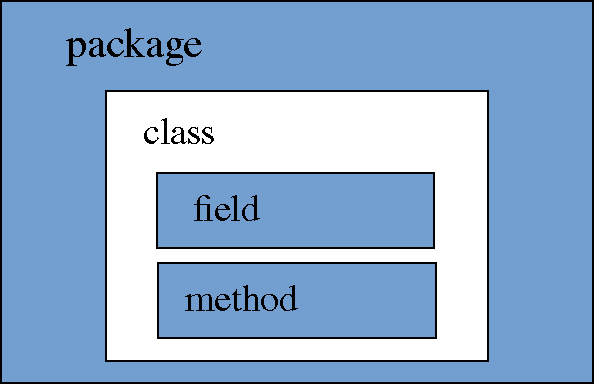
\includegraphics[width=0.45\linewidth,bb=0 0 286 185]{image/Figure_13.1.pdf}
		\caption{
			بسته‌های جاوا و سطوح رؤیت کلاس. }
	\end{figure}
	
	بسته‌های جاوا کپسوله سازی مشابه با فضای نام 
	\LTRfootnote{\lr{namespaces.}}
	\lr{C++}
	دارند که اجازه می‌دهند، اعلان‌های مرتبط با برخی اعلان‌های دیگر یک دسته شوند و از بسته‌های دیگر مخفی باشند. 
در یک برنامه جاوا، هر فیلد و متد متعلق به یک کلاس خاص است و هر کلاس بخشی از یک بسته است، همانطور که در 
	\hyperref[fig1:subsec2:sec2:chap13]{
	شکل ۱۳.۱}
	\linebreak
 آمده است، یک کلاس می‌تواند متعلق به یک بسته بی‌نام پیش فرض،‌ یا برخی از بسته‌های دیگر که در فایلی که شامل کلاس است مشخص شده‌اند، باشد.

	تمایزات رؤیت
	\LTRfootnote{visibility.}
	 در جاوا حالت‌های زیر هستند:
\begin{itemize}[nosep]
	\renewcommand{\labelitemi}{\color{gray}\scriptsize$\blacksquare$}
	\item
	\textit{
	عمومی
	\LTRfootnote{public.}
}: قابل دسترس در همه‌جا و کلاس قابل رؤیت است.
	\item\textit{
	محافظت شده
	\LTRfootnote{protected.}
}: قابل دسترس در متد‌های کلاس و هر زیر کلاسی، و همچنین به کلاس‌های دیگر در بسته یکسان. 
	\item\textit{
	خصوصی
	\LTRfootnote{private.}
}: قابل دسترس فقط در خود کلاس.
	\item\textit{
		بسته
	\LTRfootnote{package.}	
}: فابل دسترس فقط در کد با بسته یکسان، و در زیرکلاس‌های بسته‌های دیگر قابل رؤیت نیست. اعضایی که با یک مشخصه دسترسی خاصی اعلان نشده‌اند، فقط دسترسی بسته را دارند.
\end{itemize}

	به عبارت دیگر، یک متد می‌تواند به عضوی از کلاسی که به آن تعلق دارد، به اعضای غیر خصوصی همه کلاس‌ها در یک بسته، اعضای محافظت شده از کلاس‌های پدر (شامل کلاس‌های پدر در بسته‌های دیگر)، و همچنین اعضای عمومی همه کلاس‌ها در هر بسته قابل رؤیتی، مراجعه کند.
	
	نام‌های که در بسته‌های دیگر اعلان شده‌اند می‌توانند به وسیله 
	\lrInlineMono{import}
	قابل دسترس باشند، که اعلان‌های دیگر بسته‌ها را وارد می‌کند، یا اسامی واجد شرایط که در حالت زیر هستند، که  نشان می‌دهد، بسته صریحا شامل اسم است:  

\begin{latin}
	\color{steelBlue}
	$\underbrace{\texttt{java.lang}}_{\text{package}}.
	\underbrace{\texttt{String}}_{\text{class}}.
	\underbrace{\texttt{substring()}}_{\text{method}}$
\end{latin}

\subsection{
	ارث‌بری}
\label{subsec3:sec2:chap13}
	در واژه‌شناسی، یک زیر کلاس از کلاس پدر خود ارث‌بری می‌کند. که مکانیسم ارث‌بری جاوا ذاتاً مشابه ارث برای در 
	\lr{Smalltalk}، \lr{C++}
	، دیگر زبان‌های برپایه کلاس و شئ کرا است. که نحو نگارش آن در ارث‌بری مشابه 
	\lr{C++}
	، اما با کلیدواژه 
	\lrInlineMono{extends}
	است. همانطور که در این مثال نشان داده‌شده است، کلاس 
	\lrInlineMono{ColorPoint}
	از کلاس 
	\lrInlineMono{Point}
	در 
	\hyperref[subsec1:sec2:chap13]{
	زیربخش ۱۳.۲.۱} گسترش یافته است:

\begin{latin}
	\small
	\begin{lstlisting}[]
			class ColorPoint extends Point {
				// Additional fields and methods
				private Color c;
				protected void setC (Color d) {c = d;}
				public Color getC() {return c;}
				// Define constructor
				ColorPoint(int xval, Color cval) {
					super(xval); // call Point constructor
					c = cval; 
				} // initialize ColorPoint field
			};
		\end{lstlisting}
\end{latin}	

	\textit{\textbf{
		برجسته‌سازی متد
		\footnote{
			برتر سازی متد
			\lr{overriding}.}
		 و پنهان سازی فیلد‌ها.}}
	همانطور که در زبان‌های دیگر، یک کلاس تمامی فیلد‌های کلاس پدر  خود را به ارث می‌برد، بجز زمانی‌که یک فیلد یا 
	متد‌ به همان نام در زیر کلاس مورد نظر اعلان شده باشد. زمانی که یک متد در کلاس فرزند با یک متد در کلاس پدر هم نام باشد، زیرکلاس آن متد را با همان امضاء برجسته می‌کند. در یک برجسته‌سازی نوع بازگشتی متد نباید با متدی که برجسته
	\LTRfootnote{override /əʊvəˈrʌɪd/.}
	 می‌شود، با برگشت دادن نوع داده دیگر تداخل داشته باشد. یک متد برجسته شده می‌تواند به وسیله کلمه کلیدی
	 \lrInlineMono{super}
	قابل دسترس باشد. برای فیلد‌ها، یک اعلان فیلد در کلاس فرزند با اسم مشابه، تمامی فیلد‌های کلاس پدر با همان نام را پنهان می‌کند. 
	یک فیلد می‌تواند با یک نام توصیف شده  (اگر نوع آن ایستا باشد) یا با استفاده از یک عبارت دسترسی به فیلد که شامل یک تبدیل 
	به نوع کلاس پدر است و یا یا استفاده از کلیدواژه
		\lrInlineMono{super}
		 قابل دسترس باشد.

		\textit{\textbf{
			سازنده‌ها.}} جاوا ضمانت می‌کند، زمانی که یک شئ ایجاد شود سازنده آن نیز فراخوانی می‌شود. در کامپایل شدن سازنده زیرکلاس، کامپایلر چک می‌کند که حتماً سازنده کلاس پدر نیز فراخوانی شود. که اینکار به روشی خاصی که عموماً برنامه‌نویسان درنظر دارند، انجام می‌شود. بخصوص زمانی که در خط ابتدایی یک سازنده فراخوانی سازنده کلاس پدر انجام نشده است، در نتیجه کامپایلر فراخوانی تابع 
		\lrInlineMono{super()}
		را در خط اول اضافه می‌کند. البته این حالت همیشه درست عمل نمی‌کند، زیرا اگر کلاس پدر سازنده‌ای با هیچ آرگومانی
		\footnote{
		متغیره‌هایی که در ورودی تابع تعبیه می‌شوند تا بتوان به هنگام فراخونی مقادیر را به تابع فرستاد.}
	وجود نداشته باشد. فراخوانی متد 
	\lrInlineMono{super()}
	با سازنده‌های اعلان شده همخوانی نخواهد داشت، و در نتیجه باعث خطای زمان کامپایل می‌شود.
	یک استثناء در این مورد زمانی است که یک سازنده سازنده دیگری را فراخوانی کند. در این حالت سازنده اول نیازی به فراخوانی سازنده کلاس پدر را ندارد، اما سازنده دوم باید این کار را انجام دهد.
	برای مثال، اگر چنین سازنده کلاسی 
	\lrInlineMono{ColorPoint() \{ ColorPoint(0,blue);\}} 
	به کلاس 
	\lrInlineMono{ColorPoint}
	که قبلاً معرفی شد اضافه شود. در نتیجه این سازنده بدون اضافه کردن فراخوانی از سازنده کلاس پدر کامپایل می‌شود. یک اعجاب جزئی جاوا متفاوت بودن رفتار‌های ارث بری در دو متد 
	\lr{finalize}\footnote{نهایی سازی.}
	و سازنده است، که کامپایلر هیچ اجباری برای فراخوانی متد 
	\lr{finalize}
	کلاس پدر در متد 
	\lr{finalize}
	زیرکلاس وجود ندارد.
	 
	
	\textit{\textbf{
			متد نهایی
	\LTRfootnote{Final method.}
			 و کلاس‌ها.}}   جاوا دارای مکانسیم‌های جذابی برای محدود سازی زیرکلاس‌های یک کلاس دارد: به این ترتیب که یک متد یا تمام یک کلاس می‌تواند به صورت 
	\lr{final}
	  اعلان شود. اگر کلاس 
	\lr{final}
	   باشد در نتیجه، آن کلاس نمی‌توند هیچ زیر کلاسی داشته باشد. دلیل این ویژگی این است که اگر یک برنامه نویس بخواهد تمام رفتارهای تمامی شئ‌های یک نوع را تعریف کند. به دلیل اینکه یک زیرکلاس زیرنوع‌هایی ایجاد می‌کند، همانطور که در 
	\hyperref[sec3:chap13]{
	بخش ۱۳.۳} بررسی خواهد شد، اینکار نیازمند چند محدودیت بر روی زیرکلاس‌ها است. برای نشان دادن یک مثال مناسب، الگوی یکتایی
	\LTRfootnote{singleton}
	است که در بخش 
	\hyperref[sec4:chap10]{
	بخش ۱۰.۴} مورد بررسی قرار گرفت، که نشان داد چطور کلاسی طراحی کنیم که فقط یک شئ
	از کلاس بتواند ایجاد شود. این الگو سازنده را مخفی می‌کند و فقط یک تابع عمومی ایجاد می‌کند که در حین اجرای برنامه فقط یک بار می‌تواند سازنده را فراخوانی کند، اما فقط اگر هیچ زیرکلاسی متدی عمومی را برای ایجاد بیشتر از یک شئ 
	\lr{override}
	 نکند.
	اگر برنامه نویس واقعاً بخواهد الگوی یکتایی اجبار کند، باید راهی برای جلوگیری از برنامه نویسان برای تعریف زیرکلاس از یک کلاس یکتا، باشد. 
	
	 کلاس جاوا 
	\lrInlineMono{java.lang.System}
	یک مثال دیگر برای یک کلاس
	\lr{final}
	 است. این کلاس 
	\lr{final} 
	 است، تا برنامه نویسان متد‌های سیستم را 
	\lr{override}
	نکنند.
	
	به عبارت دیگر،‌ متد 
	\lr{final}
	جاوا برعکس توابع مجازی 
	\LTRfootnote{virtual functions.}
	\lr{C++}
	است: متد‌های جاوا تا زمانی که به عنوان 
	\lr{final}
	معرفی نشده باشند، می‌توانند 
	\lr{override}
	 شوند، اگر چه توابع عضو 
	\lr{C++}
	 فقط زمانی می‌توانند 
	 \lr{override}
	  شوند که به عنوان تابع مجازی در نظر گرفته شوند.
	 این قیاس خیلی دقیق نیست، هرچند که یک تابع عضو 
	 \lr{C++}
	 نمی‌تواند همزمان در یک کلاس مجازی باشد و در کلاس پدر خود و یا در کلاس مشتق شده آن مجازی نباشد، زیرا،   شکل یکسان مورد نیاز جدول مجازی برای کلاس‌های پایه و مشتق شده را نقض می‌کند. 
	
	
	\textit{\textbf{
	کلاس 
	\lr{Object}
	.}} در اصل، هر کلاس که در جاوا اعلان می‌شود یک گسترش
	\LTRfootnote{extend, inherited}
 از کلاسی دیگر است، بدین صورت که هر کلاسی که صراحتاً از کلاس دیگری ارث برای نشود به عنوان یک زیر کلاس از کلاس 
	\lr{Object}
 در نظر گرفته می‌شود.
	کلاس 
	\lrInlineMono{Object}
	یک کلاس است که هیچ کلاس پدری ندارد. کلاس 
	\lrInlineMono{Object}
	شامل متدهای زیر است که در کلاس‌های مشتق شده 
	\lrInlineMono{override}
	می‌شوند:
	
	
	\begin{itemize}[nosep]
		\renewcommand{\labelitemi}{\color{gray}\scriptsize$\blacksquare$}
		\item \lrInlineMono{GetClass}\linebreak
		که یک شئ کلاس را که نمایانگر شئ کلاس است را بر می‌گرداند.
		که می‌تواند برای پی بردن به اسم کاملاً توصیف شده کلاس، اعضای آن کلاس،  کلاس پدر بی واسطه آن و رابط‌هایی که کلاس پیاده سازی می‌کند استفاده کرد.
		\item 
		‌\lrInlineMono{ToString}
		یک رشته که نمایانگر شئ است برمی‌گرداند.
		\item ‌ 
		\lrInlineMono{equals}
		که یک ارزش از مفهوم شئ تعریف می‌کند، که مرجع مقایسه نیست.
		\item 
		‌\lrInlineMono{hasCode}
		که یک مقدار برای ذخیره سازی شئ در جداول درهم
		‌\LTRfootnote{hash table.}
		 را برمی‌گرداند.
		\item 
		‌\lrInlineMono{clone}
		که برای ایجاد یک کپی از شئ استفاده می‌شود.
		\item
		 متد‌های 
		\lrInlineMono{wait}، \lrInlineMono{notify}
		  و
		\lrInlineMono{notifyAl}
		که در برنامه نویسی همزمانی استفاده می‌شود.
		\item 
		‌\lrInlineMono{finalize}
		که درست زمانی که یک شئ از بین برود اجرا می‌شود (که در
		\hyperref[subsec1:sec2:chap13]{
		زیر بخش ۱۳.۲.۱} مرتبط با زباله روب مورد بررسی قرار گرفت.)
	\end{itemize}
 	به دلیل اینکه تمامی کلاس‌ها از متد‌های کلاس 
 	\lrInlineMono{Object}
 	ارث بری می‌کنند، در نتیجه هر شئی تمامی متد‌هایی که در بالا ذکر شد را دارد.
 	
 	\subsection{
 	کلاس‌های انتزاعی و رابط‌ها
 	}\label{subsec4:sec2:chap13}
 	مکانیزم کلاس‌های 
 	\textit{انتزاعی}
 	
 	\LTRfootnote{abstract.}
 	 زبان جاوا مشابه با زبان 
 	\lr{C++}
 	است. همانطور که ما در 
 	\hyperref[chap12]{
 	فصل ۱۲}  بررسی کردیم. کلاس انتزاعی کلاس است که تمامی متد‌های آن نیاز به پیاده سازی ندارند و از طرفی دیگر هیچ نمونه‌ای نمی‌تواند داشته باشد. جاوا از کلیدواژه 
	\lrInlineMono{abstract}
	به جای نحو 
	\lrInlineMono{"=0"}
	در 
	\lr{C++}
	استفاده می‌کند، که در کد زیر نشان داده شده است:
	
	

 	
 	همچنین جاوا یک قالب از کلاس "انتزاعی خالص" را نیز دارد که رابط
 	\LTRfootnote{interface.}
 	 نامیده می‌شود.
 	یک رابط مانند یک کلاس تعریف می‌شود، بجز اینکه تمام اعضای یک رابط باید ثابت یا متد انتزاعی باشند. یک رابط هیچ پیاده سازی مستقیمی ندارد، اما کلاس‌ها ممکن است طوری اعلان شوند که یک رابط را 
 	\lr{implement}\footnote{
 	در اینجا به عنوان یک کلمه کلیدی به کار رفته است. }
 	 کنند. به علاوه، یک رابط ممکن است به عنوان یک افزونه برای سایر کلاس‌ها باشد، که یک قالب از ارث برای رابط است.
 	
 	یکی از دلایل اینکه برنامه نویسان جاوا به جای کلاس‌های انتزاعی خالص از رابط و در زمانی که یک مفهوم تعریف شده اما پیاده سازی نشده است، استفاده می‌کنند، این است که جاوا اجازه می‌دهد که یک کلاس مجزا چندین رابط را 
 	\lr{implement}
 	 کند، درحالی که یک کلاس فقط می‌تواند یک کلاس پدر داشته باشد. در کلاس و رابط‌های زیر این  حالت به نمایش در‌آمده است. رابط 
 	 \lrInlineMono{Shape}
 	 چند ویژگی از یک شکل هندسی ساده را مشخص می کند، برای مثال هرکدام دارای یکی نقطه مرکزی و یک متد 
 	 \lrInlineMono{rotate}\footnote{
 	 	دوران.} هستند. و همچنین 
  	\lrInlineMono{Drawable}
  	چند ویژگی از شئ را که می‌تواند بر روی صفحه به نمایش درآید را نشان می‌دهد. اگر دایره یک شکل هندسی است پس همچنین می‌تواند بر روی صفحه به نمایش درآید، در نتیجه همانطور که در ادامه نشان داده شده است، کلاس 
  	\lrInlineMono{Circle}
 	 می‌تواند به نحوی اعلان شود که هر دو 
 	 \lrInlineMono{Shape} و  \lrInlineMono{Drawable} 
 	 را 
 	 \lr{implement}
 	 کند.
	\begin{latin}
		\small
		\begin{lstlisting}[]
			interface Shape {
					public Point center();
					public void rotate(float degrees);
			}
			interface Drawable {
				public void setColor(Color c);
				public void draw();
			}
			class Circle implements Shape, Drawable {
				// does not inherit any implementation
				// but must define Shape, Drawable methods
			}
		\end{lstlisting}
	\end{latin}	
برخلاف ارث بری چندگانه در 
\lr{C++}
(که در 
\hyperref[sec5:chap12]{
	بخش ۱۲.۵} بررسی شد)، هیچ مشکل تصادم اسم در رابط‌های جاوا وجود ندارد. به طور خاص، فرض کنید که
	 دو رابط 
	 \lrInlineMono{Shape}
	 و
	 \lrInlineMono{Circle}
	 تعریف شده در قبل  هر دو متد 
	 \lrInlineMono{Size}
	 را پیاده سازی کرده‌اند. اگر متد‌های 
	 \lrInlineMono{Size}
	 هردو تعداد آرگومان با نوع یکسان داشته باشند. در نتیجه کلاس 
	 \lrInlineMono{Circle}
	 باید یک متد 
	 \lrInlineMono{Size}
	 با این با تعداد آرگومان و نوع آرگومان موجود در دو رابط پیاده سازی کند. از طرف دیگر، اگر دو متد 
	 \lrInlineMono{Size}
	 آرگومان‌هایی با تعداد و یا نوع متمایز داشته باشند، در نتیجه آنها به عنوان دو متد متفاوت در نظر گرفته شده و کلاس 
	 \lrInlineMono{Circle}
	 باید متد 
	 \lrInlineMono{Size}
	  را برای هر کدام را پیاده سازی کند. به این خاطر که جستجوی متد جاوا از نام و تعداد و نوع آرگومان‌ها برای انتخاب کد متد استفاده می‌کند، دو متد با نام‌های  یکسان در زمان جستجوی متد‌ها به صورت مجزا تلقی می‌شوند.
	 
	\section{
	نوع‌ها و زیر نوع‌های جاوا }
	\label{sec3:chap13}
	\subsection{
	طبقه بندی نوع‌ها}
	\label{subsec1:sec3:chap13}
	
	نوع‌های جاوا در دو دسته تقسیم می‌شوند: نوع‌های اولیه و نوع‌های ارجاعی. هشت نوع اولیه به نوع 
	\lrInlineMono{boolean}
	و هفت نوع دیگر از انواع عددی در فرم 
	\lrInlineMono{integers byte}، \lrInlineMono{short}
	، \lrInlineMono{int}، \lrInlineMono{long}، \lrInlineMono{char}
	و نوع‌های اعشاری
	\lrInlineMono{float} 
	و 
	\lrInlineMono{double}
	هستند. سه نوع در انواع ارجاعی وجود دارند، نوع‌های 
	\lrInlineMono{class}، \lrInlineMono{interface}
	(که اخیراً بحث شد) و نوع آرایه. و همچنین نوع خاص 
	\lrInlineMono{null}
	هم موجود است. مقادیر یک نوع ارجاعی یک ارجاع به شئ است (که شامل آرایه نیز می‌شود). تمام اشیاء، شامل آرایه‌ها، متدهای 
	کلاس 
	\lrInlineMono{Object}
	را پشتیبانی می‌کنند. 
	
	رابطه زیر نوع بین نوع‌های اصلی در 
	\hyperref[fig1:subsec1:sec3:chap13]{
		شکل ۱۳.۲} به نمایش در‌آمده‌اند، که شامل رابط‌های 
	\lrInlineMono{Shape} 
	 و کلاس‌های
	\lrInlineMono{Circle} و \lrInlineMono{Square}
	تا نشان بدهند که چطور کلاس‌ها و رابط‌های تعریف شده توسط کاربر در تصویر گنجانده شده‌اند.
	مابقی نوع‌های پیش تعریف شده مانند:
	\lrInlineMono{Strings}، \lrInlineMono{ClassLoader} و \lrInlineMono{Thead}
	در جایگاهی مانند
	\lrInlineMono{Exception}
	در این شکل دارند.
	 
	
	
	
	
	
\lr{	
	interface types (subsequently discussed), and array types. There is also a special null
	type. The values of a reference type are references to objects (which include arrays).
	All objects, including arrays, support the methods of class Object .
	The subtyping relationships between the main families of types are illustrated in
	Figure 13.2, which includes a Shape interface and Circle and Square classes to show
	how user-defined classes and interfaces fit into the picture. Other predefined types
	such as String , ClassLoader , and Thread occupy positions similar to that of Exception
	in this figure.
	-> Object[] is the type of arrays of objects, and similarly for array types
	Shape[] , Circle[] , and Square[] .
	Although it is standard Java terminology to call Object and its subtypes reference
	types, this may be slightly confusing. Although C++ distinguishes Object from Object * ,
	there are no explicit pointer types in Java. Instead, the difference between a pointer
	to an object and an object itself is implicit, with pointer dereferencing combined with
	operations like method invocation and field access. If T is a reference type, then a
	variable x of type T is a reference to T objects; in C++ the variable x would have type
	T* . Because there is no explicit way to dereference x to get a value of type T , Java
	does not have a separate type for objects not referred to by pointer.
}
	
	\begin{figure}[!h]
		\label{fig1:subsec1:sec3:chap13}
		\centering
		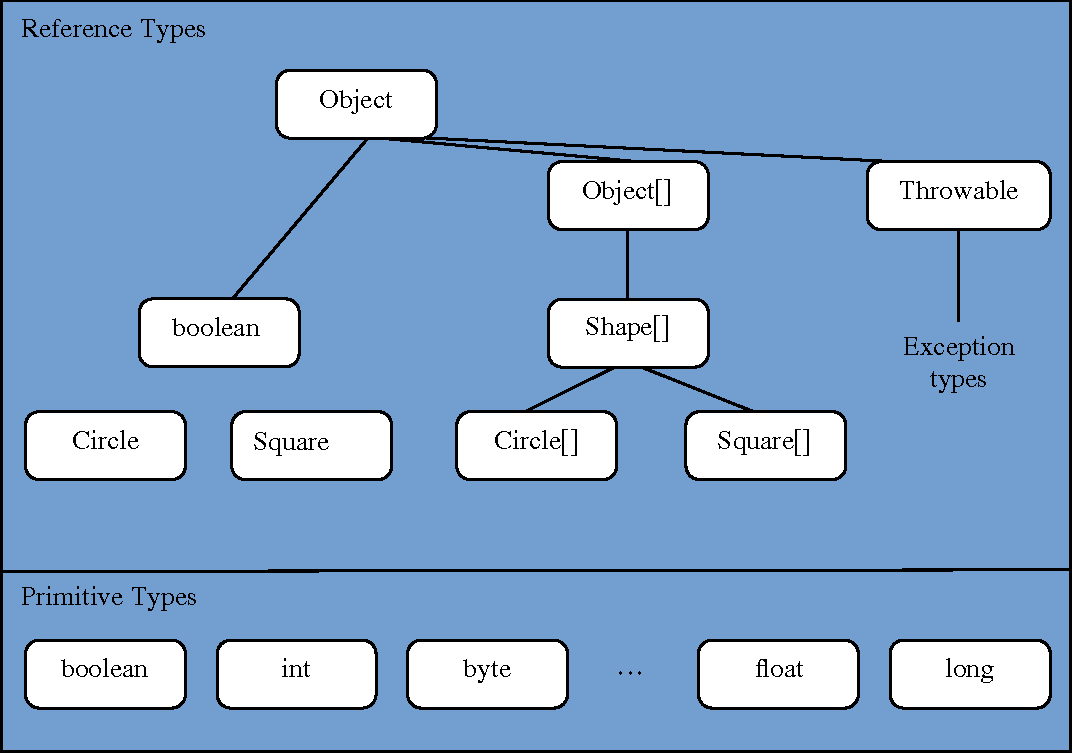
\includegraphics[width=0.9\linewidth,bb=0 0 514.57 361.51]{image/Figure_13.2.pdf}
		\caption{
			طبقه بندی نوع‌ها در جاوا.}
	\end{figure}

\end{document}